%%%%%%%%%%%%%%%%%%%%%%%%%%%%%%%%%%%%%%%%%%
% Master Thesis 
% Polina Polunina
% October 2022 
%
% License:
% CC-BY-SA 4.0 -- Creative Commons Attribution-ShareAlike 4.0 International
% https://creativecommons.org/licenses/by-sa/4.0/legalcode
%%%%%%%%%%%%%%%%%%%%%%%%%%%%%%%%%%%%%%%%%%
\section{Appendix} \label{sec:appendix}

    \subsection{Galaxy tool wrappers} \label{sec:appendix:galaxy-wrappers}
    Macros for collection of related Freyja tool wrappers: \\
    \url{https://github.com/galaxyproject/tools-iuc/blob/master/tools/freyja/macros.xml}\\
    Tool wrapper for Freyja: Call variants and get sequencing depth information: \\
    \url{https://github.com/galaxyproject/tools-iuc/blob/master/tools/freyja/freyja_variants.xml}\\
    Tool wrapper for Freyja: Bootstrapping method: \\
    \url{https://github.com/galaxyproject/tools-iuc/blob/master/tools/freyja/freyja_boot.xml}\\
    Tool wrapper for Freyja: Demix lineage abundances: \\
    \url{https://github.com/galaxyproject/tools-iuc/blob/master/tools/freyja/freyja_demix.xml}\\
    Tool wrapper for Freyja: Aggregate and visualize demixed results: \\
    \url{https://github.com/galaxyproject/tools-iuc/blob/master/tools/freyja/freyja_aggregate_plot.xml}\\
    \\
    Macros for collection of related Cojac tool wrappers: \\
    \url{https://github.com/galaxyproject/tools-iuc/blob/master/tools/cojac/macros.xml}\\
    Tool wrapper for Cojac: mutbamscan: \\
    \url{https://github.com/galaxyproject/tools-iuc/blob/master/tools/cojac/cooc_mutbamscan.xml}\\
    Tool wrapper for Cojac: tabmut: \\
    \url{https://github.com/galaxyproject/tools-iuc/blob/master/tools/cojac/cooc_tabmut.xml}\\
    Tool wrapper for Cojac: pubmut: \\
    \url{https://github.com/galaxyproject/tools-iuc/blob/master/tools/cojac/cooc_pubmut.xml}
    
    \subsection{Published Galaxy workflows} \label{sec:appendix:galaxy-wfs}
    The workflow for SARS-CoV-2 wastewater Illumina-sequenced ARTIC data analysis: \\
    \url{https://usegalaxy.eu/u/polina/w/ww-sars-cov-2-artic-pe-workflow} \\
    
    The workflow for SARS-CoV-2 wastewater Illumina-sequenced metatranscriptomics data analysis: \\
    \url{https://usegalaxy.eu/u/polina/w/ww-sars-cov-2-metatranscriptomics-pe-workflow} \\

    \subsection{Galaxy histories} \label{sec:appendix:galaxy-hist}
    \subsubsection{Galaxy history links for Freyja-based branch on real datasets}
    California, US (PRJNA661613): \\
   \url{https://usegalaxy.eu/u/polina/h/sf-dataset-prjna661613-covid-19-variation-analysis-on-wgs-pe-data}\\
    Wales and Northwest England, UK (PRJEB42191): \\
    \url{https://usegalaxy.eu/u/polina/h/uk-dataset-COJAC-prjeb42191-covid-19-variation-analysis-on-artic-pe-data-1}\\
    Ontario, Canada (PRJNA824537): \\
    \url{https://usegalaxy.eu/u/polina/h/ca-dataset-freyja-prjna824537-covid-19-variation-analysis-on-artic-pe-data}\\
    Washington, US (PRJNA765346): \\
    \url{https://usegalaxy.eu/u/polina/h/us-dataset-freyja-prjna765346-covid-19-variation-analysis-on-artic-pe-data-1-1-1-1}

    \subsubsection{Galaxy history links for COJAC-based branch on real datasets}
    Wales and Northwest England, UK (PRJEB42191): \\
    \url{https://usegalaxy.eu/u/polina/h/uk-dataset-COJAC-prjeb42191-covid-19-variation-analysis-on-artic-pe-data-1}\\
    Ontario, Canada (PRJNA824537): \\
    \url{https://usegalaxy.eu/u/polina/h/ca-dataset-COJAC-prjna824537-covid-19-variation-analysis-on-artic-pe-data}\\
    Washington, US (PRJNA765346): \\
    \url{https://usegalaxy.eu/u/polina/h/us-dataset-COJAC-prjna765346-covid-19-variation-analysis-on-artic-pe-data}
    
    \subsection{Computation of overall lineage abundances for Freyja output} \label{sec:appendix:recompute-freyja}
    Python script to compute the overall lineage abundances proportions of considered lineages in mock dataset for Freyja output:\\
    \url{https://github.com/PlushZ/mthesis-sars-ww-galaxy/blob/main/overall-lineage-abundances-freyja.ipynb}
    
    \subsection{Visualisations of results on mock dataset} \label{sec:appendix:mock-visualize}
    Jupyter notebooks for visualisations of results on mock dataset: \\
    \url{https://github.com/PlushZ/mthesis-sars-ww-galaxy/blob/main/mock-benchmark-visualizations.ipynb} 
    
    \subsection{Visualisations of results on real-world dataset} \label{sec:appendix:real-visualize}
    Jupyter notebooks for visualisations of real-world datasets for SARS-CoV-2 wastewater surveillance and results on real-world datasets: \\
    \url{https://github.com/PlushZ/mthesis-sars-ww-galaxy/blob/main/realworld-benchmark-visualizations.ipynb}
    
    \subsection{This document itself in Latex} \label{sec:appendix:real-visualize}
    This thesis itself is written in Latex and is stored in GitHub repository: \\
    \url{https://github.com/PlushZ/master-thesis-latex}


    \subsection{Further figures}
        \subsubsection{Existing Galaxy workflows that were not changed} \label{sec:appendix:figures:wfs}
        Other existing Galaxy workflows for SARS-CoV-2 clinical data surveillanve that were not taken as a basis for improvement and repurposing in this thesis are presented in \cref{fig:further:ont-wf} and \cref{fig:further:illumina-wf}.
        \begin{landscape}
        \centering\vspace*{\fill}
        \begin{figure}[ht!]
        	\centering
            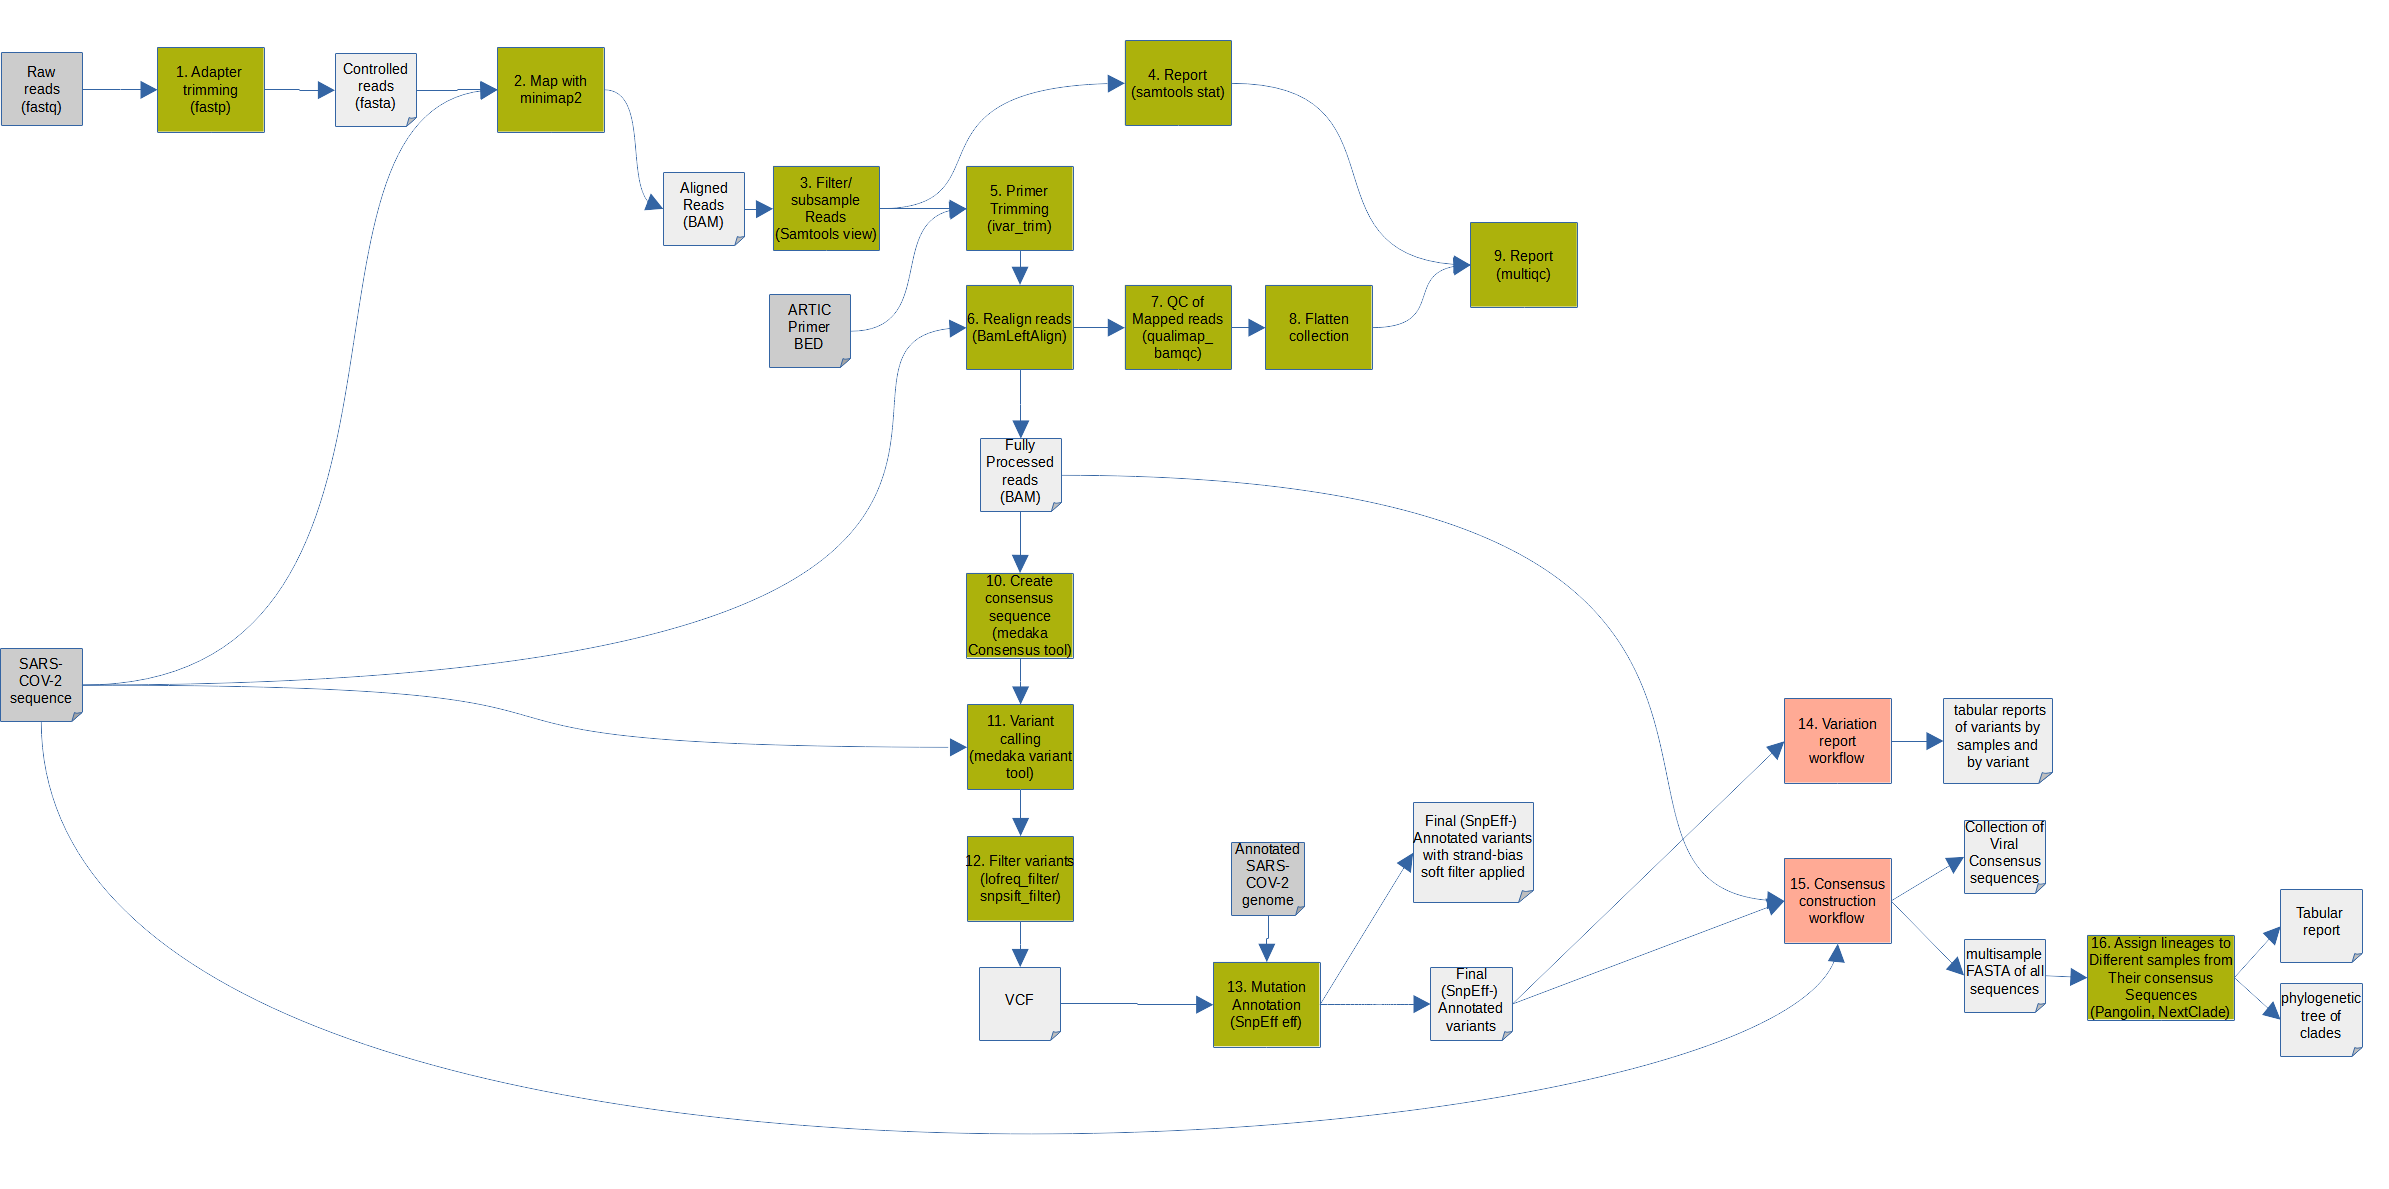
\includegraphics[width=1.4\textwidth]{figures/further/further-ont-wf.png}
            \captionof{figure}{One of four existing Galaxy workflow for SARS-CoV-2 clinical data surveillance for single-end reads data extracted with amplicon-based technique and sequenced with Nanopore sequencing approach.}
            \label{fig:further:ont-wf}
        \end{figure}
        \begin{figure}[ht!]
        	\centering
            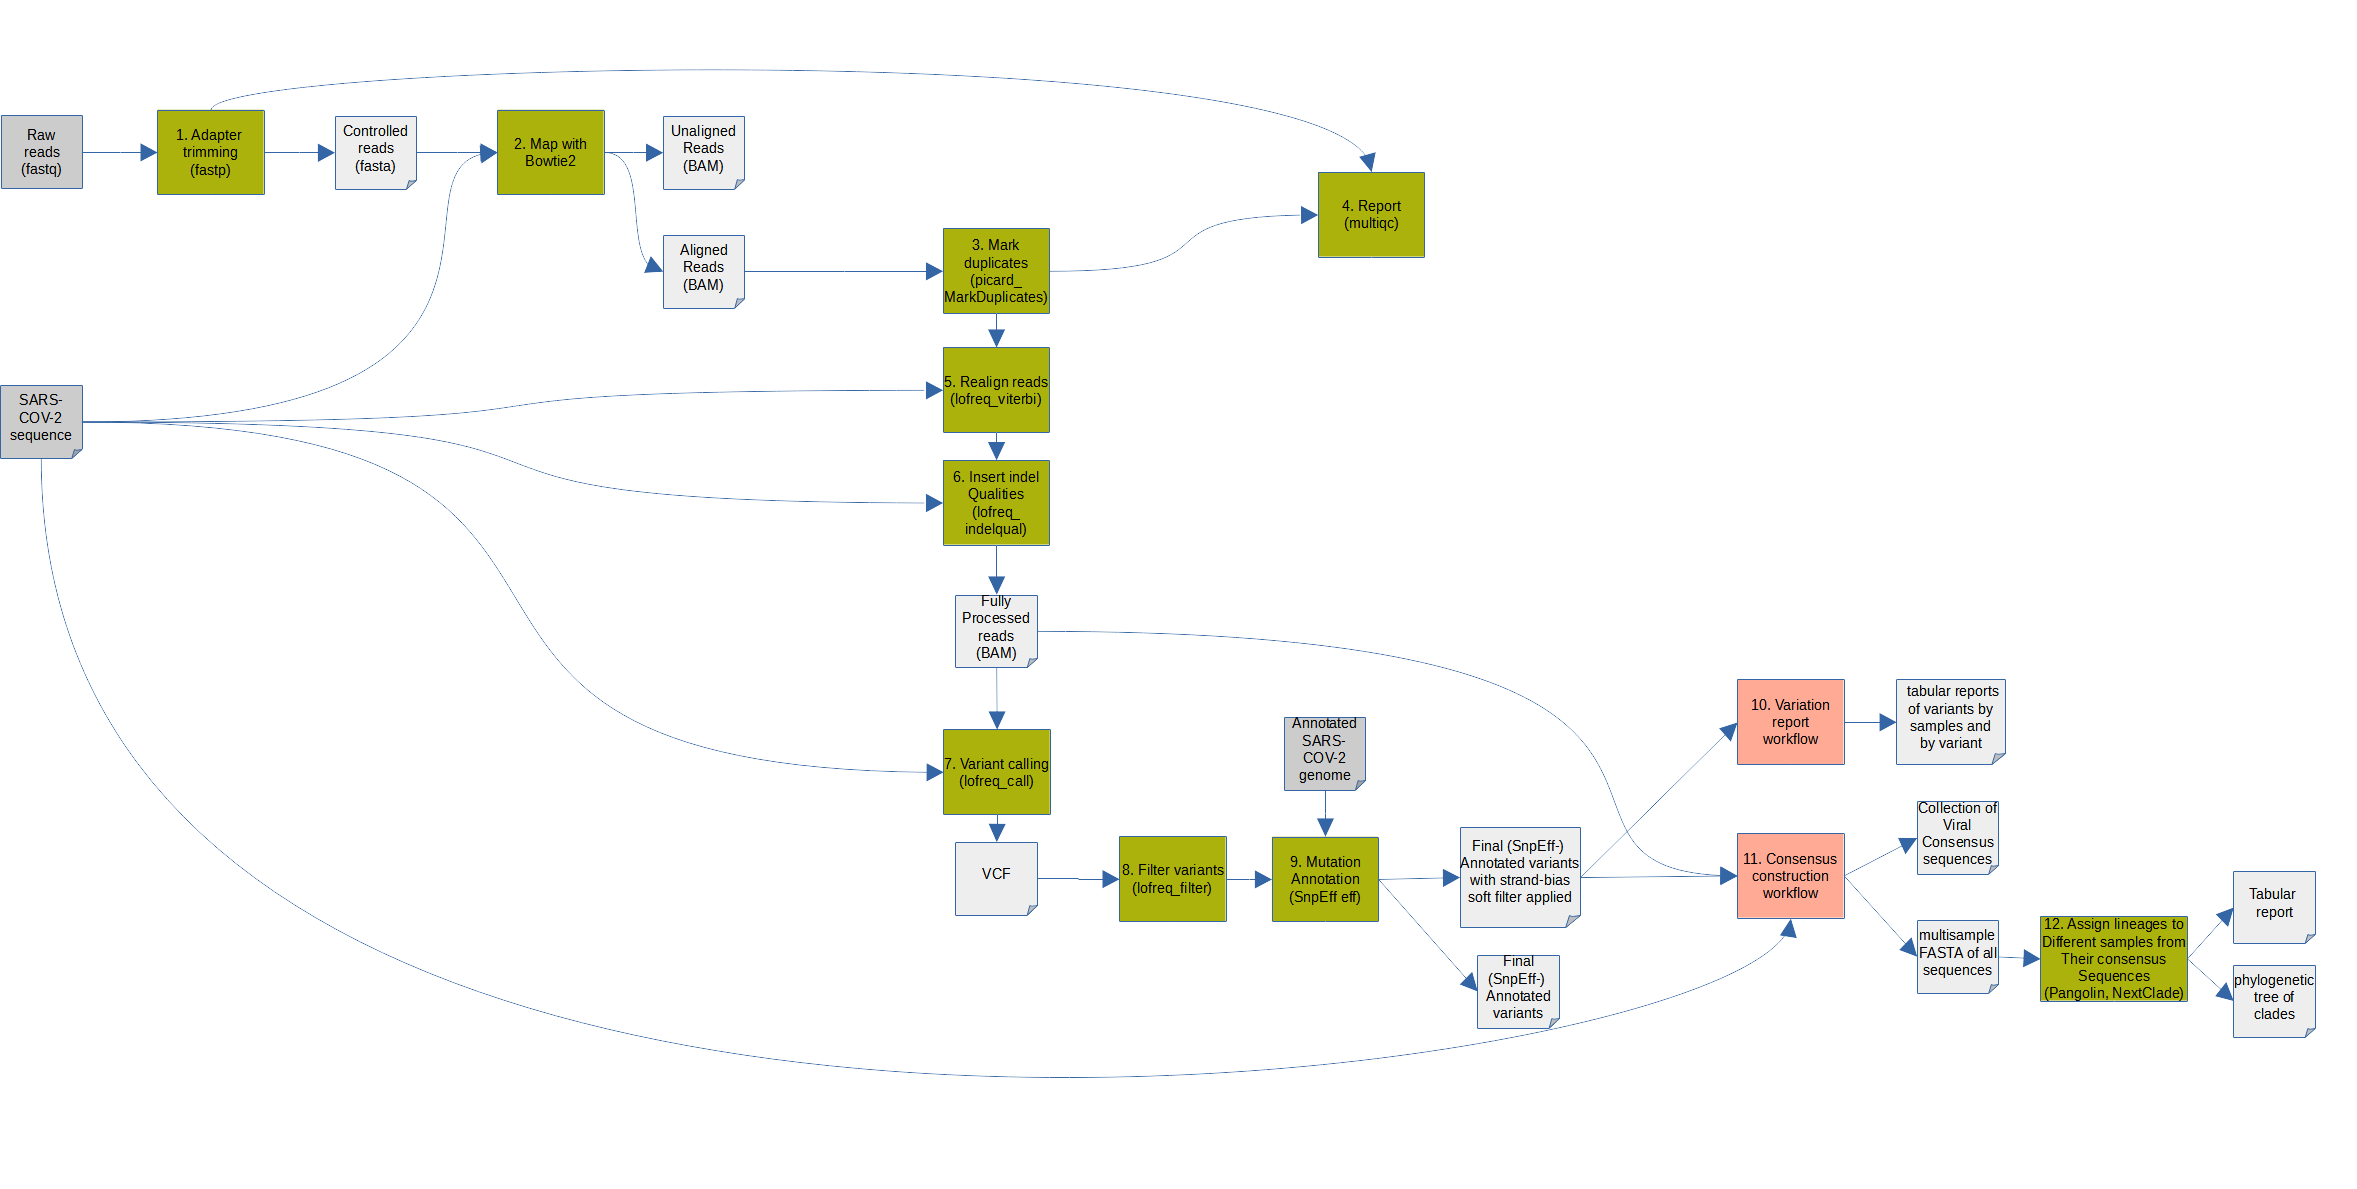
\includegraphics[width=1.4\textwidth]{figures/further/further-illumina-wf.png}
            \captionof{figure}{One of four existing Galaxy workflow for SARS-CoV-2 clinical data surveillance for single-end reads data extracted with metatranscriptomic-based technique and sequenced with Illumina sequencing approach.}
            \label{fig:further:illumina-wf}
        \end{figure}
        \vfill
        \end{landscape}
        
        \subsubsection{Comparison of lineage proportions detected by tools with expected proportion} 
        \paragraph{Comparison of lineage proportions in all mock samples} \label{sec:appendix:figures:parallel-all}
        \Cref{fig:further:parallel-delta-all}, \cref{fig:further:parallel-ba1-all} and \cref{fig:further:parallel-ba2-all} depict parallel coordinates for all samples considering only detection of Delta, BA.1, and BA.2 lineage respectively by Freyja and COJAC.
        \begin{figure}[H]
        	\centering
            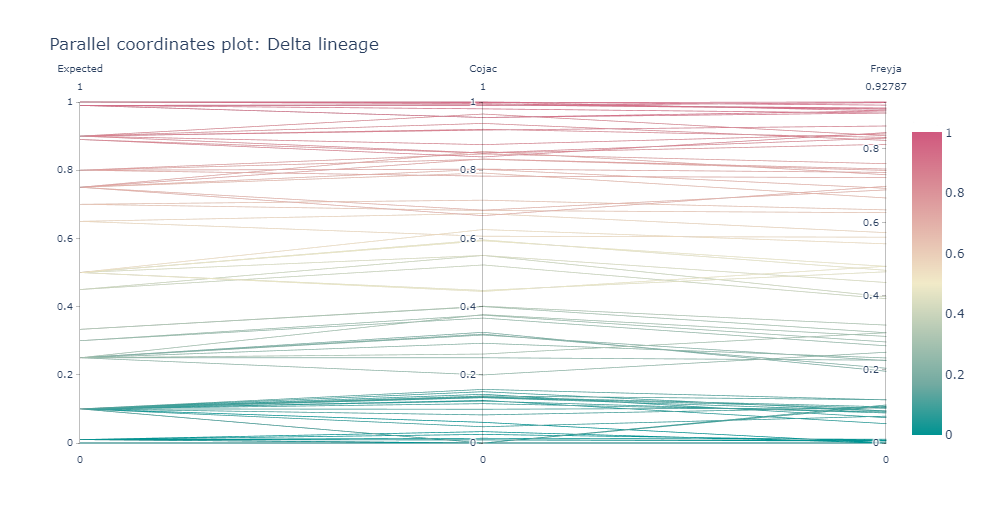
\includegraphics[width=0.8\textwidth]{figures/further/pc-delta-all.png}
            \captionof{figure}{Parallel coordinates plot for all samples that compare Delta lineage proportions detected by Freyja and COJAC with each other as well as with expected proportion. Left axis represents expected proportion of Delta, middle axis represents proportion of Delta lineage detected by COJAC, while right axis represents proportion of Delta lineage detected by Freyja}
            \label{fig:further:parallel-delta-all}
        \end{figure}
        \begin{figure}[H]
        	\centering
            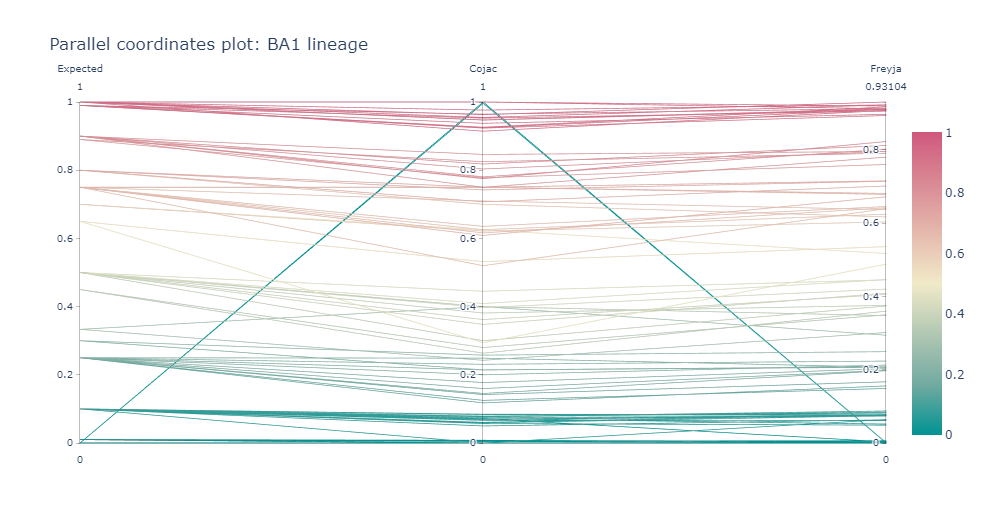
\includegraphics[width=0.8\textwidth]{figures/further/pc-ba1-all.png}
            \captionof{figure}{Parallel coordinates plot for all samples that compare BA.1 lineage proportions detected by Freyja and COJAC with each other as well as with expected proportion. Left axis represents expected proportion of BA.1, middle axis represents proportion of BA.1 lineage detected by COJAC, while right axis represents proportion of BA.1 lineage detected by Freyja}
            \label{fig:further:parallel-ba1-all}
        \end{figure}
        \begin{figure}[H]
        	\centering
            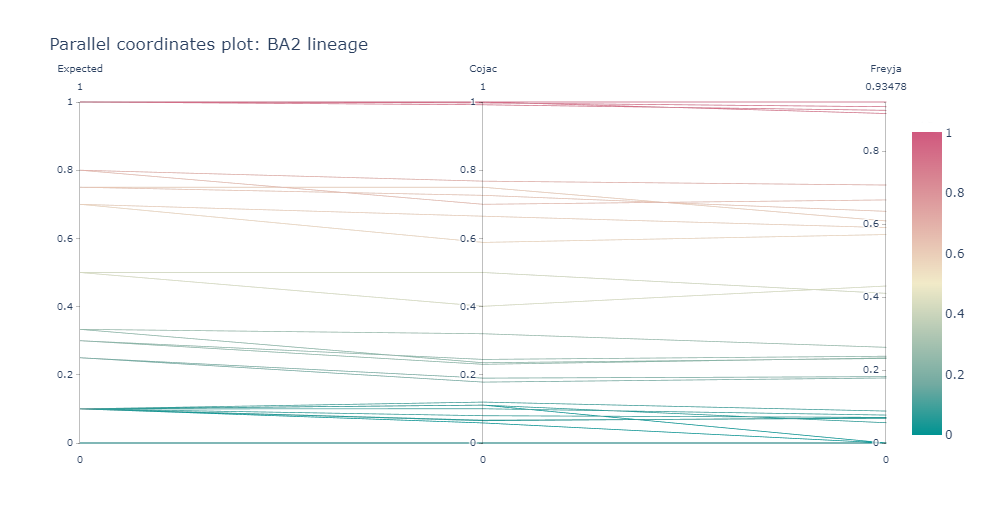
\includegraphics[width=0.8\textwidth]{figures/further/pc-ba2-all.png}
            \captionof{figure}{Parallel coordinates plot for all samples that compare BA.2 lineage proportions detected by Freyja and COJAC with each other as well as with expected proportion. Left axis represents expected proportion of BA.2, middle axis represents proportion of BA.2 lineage detected by COJAC, while right axis represents proportion of BA.2 lineage detected by Freyja}
            \label{fig:further:parallel-ba2-all}
        \end{figure}
        
        \paragraph{Comparison of lineage proportions in mock samples with two lineages expected} \label{sec:appendix:figures:parallel-twolin}
        \Cref{fig:further:parallel-delta-twolin}, \cref{fig:further:parallel-ba1-twolin} and \cref{fig:further:parallel-ba2-twolin} depict parallel coordinates for "two lineages" group of samples considering only detection of Delta, BA.1, and BA.2 lineage respectively by Freyja and COJAC. Although, for the "two lineages" group of samples, it is not that reasonable to separate graphs into different lineages but focus on the ratio between two expected lineages. Even though, detected proportion of certain expected lineage was worthwhile to to have a look at. Thus, parallel coordinates graphs were generated in the way of one graph per lineage.
        \begin{figure}[H]
        	\centering
            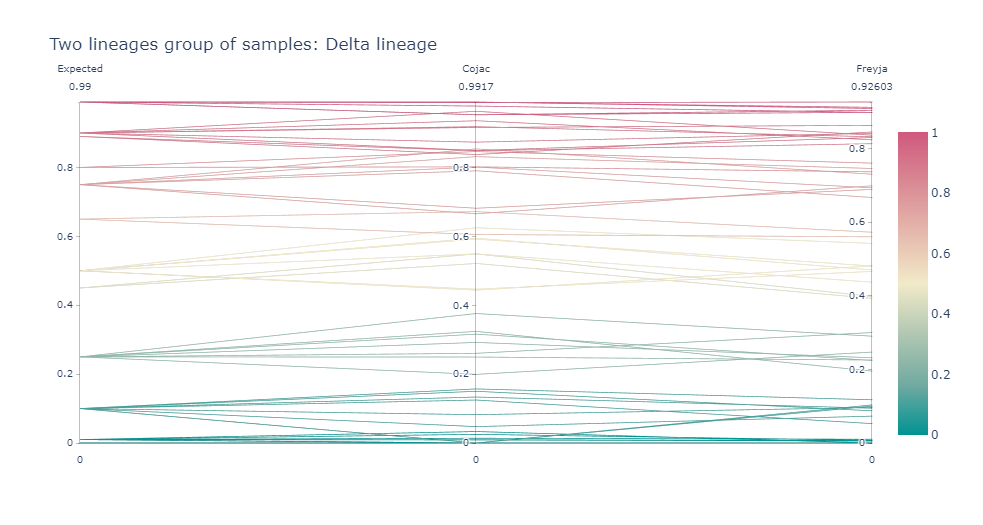
\includegraphics[width=0.8\textwidth]{figures/further/pc-twolin-delta.png}
            \captionof{figure}{Parallel coordinates plot for "two lineages group" of samples that compare Delta lineage proportions detected by Freyja and COJAC with each other as well as with expected proportion. Left axis represents expected proportion of Delta, middle axis represents proportion of Delta lineage detected by COJAC, while right axis represents proportion of Delta lineage detected by Freyja}
            \label{fig:further:parallel-delta-twolin}
        \end{figure}
        \begin{figure}[H]
        	\centering
            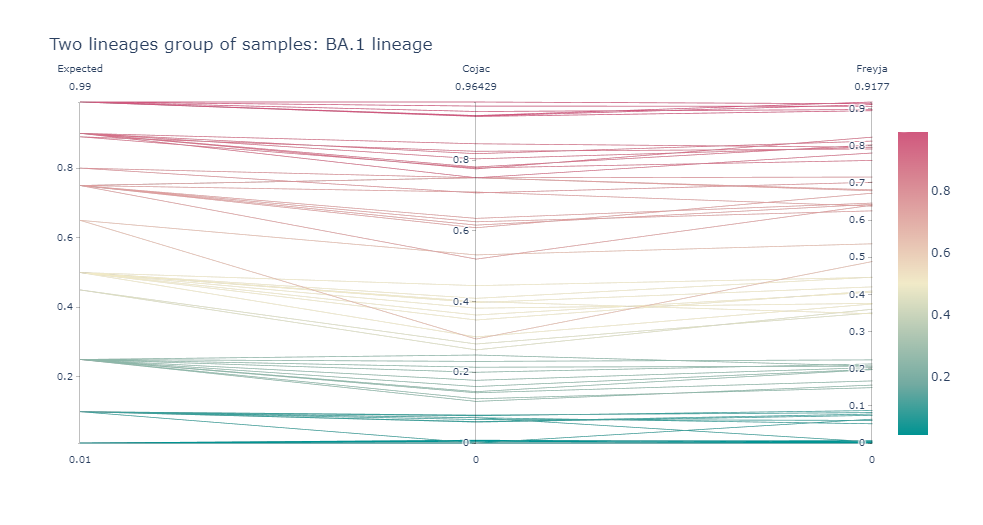
\includegraphics[width=0.8\textwidth]{figures/further/pc-twolin-ba1.png}
            \captionof{figure}{Parallel coordinates plot for "two lineages group" of samples that compare BA.1 lineage proportions detected by Freyja and COJAC with each other as well as with expected proportionfor "two lineages group" of samples. Left axis represents expected proportion of BA.1, middle axis represents proportion of BA.1 lineage detected by COJAC, while right axis represents proportion of BA.1 lineage detected by Freyja}
            \label{fig:further:parallel-ba1-twolin}
        \end{figure}
        \begin{figure}[H]
        	\centering
            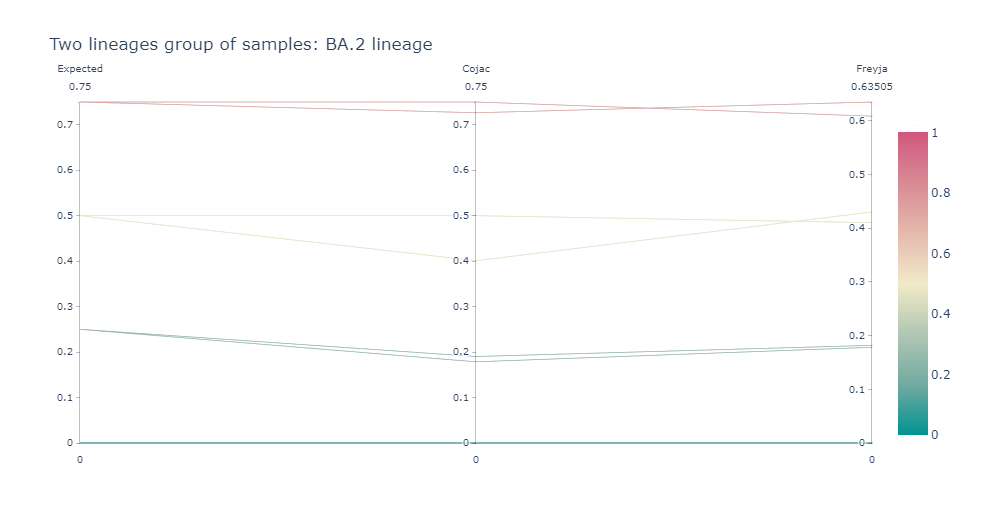
\includegraphics[width=0.8\textwidth]{figures/further/pc-twolin-ba2.png}
            \captionof{figure}{Parallel coordinates plot for "two lineages group" of samples that compare BA.2 lineage proportions detected by Freyja and COJAC with each other as well as with expected proportion for "two lineages group" of samples. Left axis represents expected proportion of BA.2, middle axis represents proportion of BA.2 lineage detected by COJAC, while right axis represents proportion of BA.2 lineage detected by Freyja}
            \label{fig:further:parallel-ba2-twolin}
        \end{figure}
        
        \subsubsection{Example of different types of plots for one mock sample} 
        \Cref{fig:further:bar-s1}, \cref{fig:further:pc-s1} and \cref{fig:further:line-s1} show plots generated per sample to make detailed observations. The example for the sample1 is provided below. However, these graphs were constructed for every sample during this master thesis. Types of plots that were generated per one sample: i) bar plot (\cref{fig:further:bar-s1}); ii) parallel coordinates plot (\cref{fig:further:pc-s1}); iii) line plot (\cref{fig:further:line-s1}), to look at absolute values of lineage proportion against scaled values in parallel coordinates. The comparison with expected lineage proportions was included in these plots.
.
        \begin{figure}[H]
        	\centering
            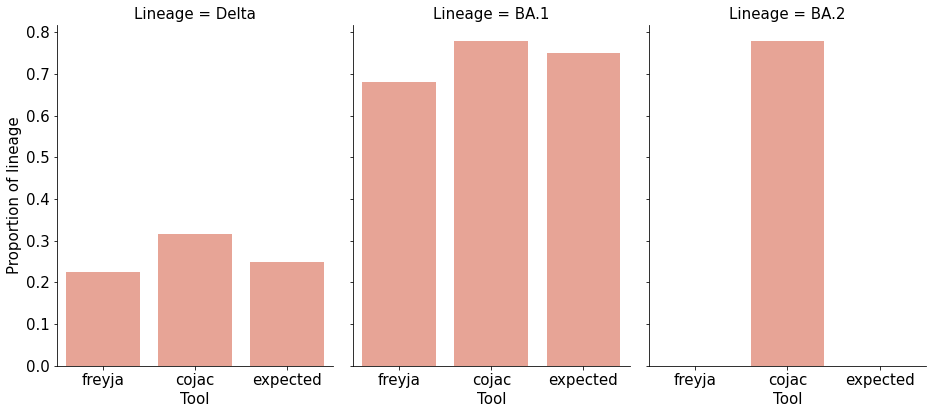
\includegraphics[width=0.8\textwidth]{figures/further/bar-s1.png}
            \captionof{figure}{Bar plot for sample 1.}
            \label{fig:further:bar-s1}
        \end{figure}
        \begin{figure}[H]
        	\centering
            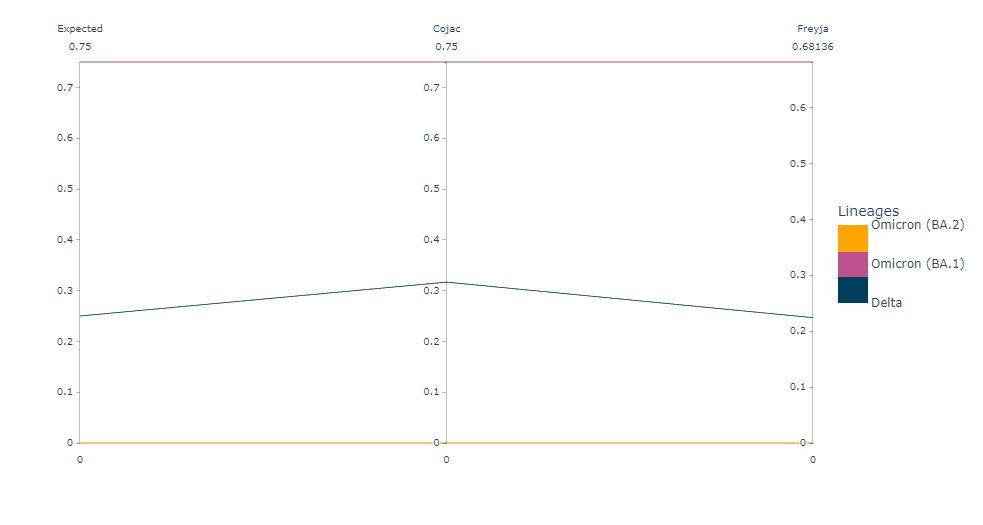
\includegraphics[width=0.8\textwidth]{figures/further/pc-s1.png}
            \captionof{figure}{Parallel coordinates plot for sample 1}
            \label{fig:further:pc-s1}
        \end{figure}
        \begin{figure}[H]
        	\centering
            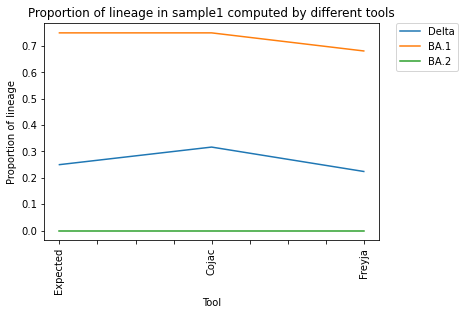
\includegraphics[width=0.8\textwidth]{figures/further/line-s1.png}
            \captionof{figure}{Line plot for sample 1}
            \label{fig:further:line-s1}
        \end{figure}
        
       \subsubsection{Distribution of lineages proportions detected by Lineagespot across all mock samples}  
        \Cref{fig:further:dist-ls} represents the proportions of every lineage detected by Lineagespot on mock dataset. Observed that most of the samples, more than 50\%, according to Lineagespot, carry a small proportion, no more than 0.15, of lineage abundance, while higher proportions of all 3 lineages are present in less amount of samples.
        \begin{figure}[H]
        	\centering
            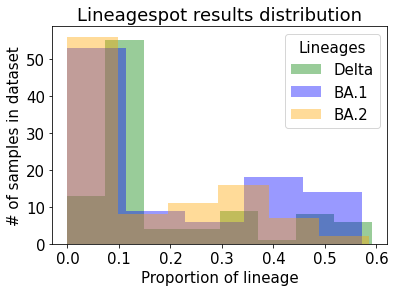
\includegraphics[width=0.5\textwidth]{figures/further/distr-lineagespot.png}
            \captionof{figure}{All three considered lineages (Delta, BA.1, BA.2) proportion distribution among results detected by Lineagespot on mock dataset.}
            \label{fig:further:dist-ls}
        \end{figure}
        
    \subsection{Supplementary tables}
        \subsubsection{Freyja aggregated demixed data} \label{sec:appendix:tabs:freyja}
\begin{landscape}
            \centering\vspace*{\fill}
                \begin{table}[ht!]
                \tiny
                \begin{tabular}{l|l|l|l|l|l}
                            &summarized&lineages&abundances&resid&coverage\\ \hline
                SRR12596165.fastq&"[('Other', 0.9999999999972105)]"&\multicolumn{1}{m{5cm}|}{B.10 B.47 B.23 B.26 B.1.14 B.20 B}&\multicolumn{1}{m{5cm}|}{0.14285714 0.14285714 0.14285714 0.14285714 0.14285714 0.14285714 0.14285714}&2.63E-12&1.926550271\\ \hline
                SRR12596166.fastq&"[('Other', 0.9999999999983175)]"&\multicolumn{1}{m{5cm}|}{B.1.1.174 B.10 B.47 B.23 B.26 B.1.14 B.20 B}&\multicolumn{1}{m{5cm}|}{0.55555600 0.06349200 0.06349200 0.06349200 0.06349200 0.06349200 0.06349200 0.06349200}&1.162673375&1.926550271\\ \hline
                SRR12596167.fastq&"[('Other', 0.9999999999996593)]"&\multicolumn{1}{m{5cm}|}{B.10 B.47 B.23 B.26 B.1.14 B.20 B}&\multicolumn{1}{m{5cm}|}{0.14285714 0.14285714 0.14285714 0.14285714 0.14285714 0.14285714 0.14285714}&0.75&1.926550271\\ \hline
                SRR12596168.fastq&"[('Other', 0.9999999999582964)]"&\multicolumn{1}{m{5cm}|}{B.1.1.174 B.1.1.161 B.1.564 B.1.12 B.1.607 B.1.413 B.1.324 B.1.453 B.1.1.372 B.1.1 B.1.1.92 B.1.1.294 B.1.1.180 B.1.1.43 B.1.1.59 B.1.1.463 B.1.1.402 B.1.1.10 B.1.1.208 B.1.1.61 B.10 B.47 B.23 B.26 B.1.14 B.20 B}&\multicolumn{1}{m{5cm}|}{0.27027000 0.08080800 0.05555550 0.05555550 0.05555550 0.05555550 0.05555550 0.05555550 0.02377383 0.02377383 0.02377383 0.02377383 0.02377383 0.02377383 0.02377383 0.02377383 0.02377383 0.02377383 0.02377383 0.02377383 0.00432900 0.00432900 0.00432900 0.00432900 0.00432900 0.00432900 0.00432900}&0.4968557797&1.926550271\\ \hline
                SRR12596169.fastq&"[('Other', 0.9999999999979102)]"&\multicolumn{1}{m{5cm}|}{B.1.111 B.1.1.174 B.1.479 B.1.22 B.1.533 B.1.12 B.1.607 B.1.453 B.1.324 B.1.413 B.1.564 B.1.199 B.1.378 B.1.201 B.1.215 B.1}&\multicolumn{1}{m{5cm}|}{0.14432305 0.14285700 0.09853229 0.06999717 0.05158700 0.04640292 0.04640292 0.04640292 0.04640292 0.04640292 0.04640292 0.04285720 0.04285720 0.04285720 0.04285720 0.04285720}&0.7140985235&1.926550271\\ \hline
                SRR12596170.fastq&"[('Other', 0.9999999999987905)]"&\multicolumn{1}{m{5cm}|}{B.1.533 B.1.370 B.1.301 B.1.424 B.1.111 B.1.479 B.1.201 B.1.378 B.1.199 B.1.215 B.1 B.1.22 B.1.453 B.1.324 B.1.413 B.1.607 B.1.12 B.1.564 B.1.1.161 B.10 B.47 B.23 B.26 B.1.14 B.20 B}&\multicolumn{1}{m{5cm}|}{0.15773800 0.11717199 0.11641401 0.11641400 0.05154872 0.03906387 0.03904760 0.03904760 0.03904760 0.03904760 0.03904760 0.03189755 0.01718081 0.01718081 0.01718081 0.01718081 0.01718081 0.01718081 0.00892900 0.00892857 0.00892857 0.00892857 0.00892857 0.00892857 0.00892857 0.00892857}&0.4778312073&1.926550271\\ \hline
                SRR12596171.fastq&"[('Other', 0.9979179208943117)]"&\multicolumn{1}{m{5cm}|}{B.1.509 B.1.12 B.1.607 B.1.453 B.1.324 B.1.413 B.1.564 B.10 B.47 B.23 B.26 B.1.14 B.20 B}&\multicolumn{1}{m{5cm}|}{0.87096800 0.01560282 0.01560282 0.01560282 0.01560282 0.01560282 0.01560282 0.00476186 0.00476186 0.00476186 0.00476186 0.00476186 0.00476186 0.00476186}&0.3834278298&1.926550271\\ \hline
                SRR12596172.fastq&"[('Other', 0.9999999999983878)]"&\multicolumn{1}{m{5cm}|}{B.1.301 B.1.424 B.1.370 B.1.1.174 B.1.453 B.1.12 B.1.607 B.1.324 B.1.413 B.1.564 B.47 B.20 B.1.14 B.26 B.23 B B.10 B.1.533 B.1.111 B.1.22 B.1.479}&\multicolumn{1}{m{5cm}|}{0.27497564 0.27497564 0.27312572 0.03731300 0.01588226 0.01588226 0.01588226 0.01588226 0.01588226 0.01588226 0.00529100 0.00529100 0.00529100 0.00529100 0.00529100 0.00529100 0.00529100 0.00367100 0.00125773 0.00118732 0.00116342}&0.54272957&1.926550271\\ \hline
                SRR12596173.fastq&"[('Other', 0.9999999999972105)]"&\multicolumn{1}{m{5cm}|}{B.10 B.47 B.23 B.26 B.1.14 B.20 B}&\multicolumn{1}{m{5cm}|}{0.14285714 0.14285714 0.14285714 0.14285714 0.14285714 0.14285714 0.14285714}&2.63E-12&1.926550271\\ \hline
                SRR12596174.fastq&"[('Other', 0.999999999979265)]"&\multicolumn{1}{m{5cm}|}{B.1.509 B.1.2 B.1.370 B.1.301 B.1.424 B.1.324 B.1.564 B.1.413 B.1.453 B.1.607 B.1.12 B.1.596 B.47 B.20 B.1.14 B.26 B.23 B B.10 B.1 B.1.215 B.1.201 B.1.378 B.1.199}&\multicolumn{1}{m{5cm}|}{0.28000000 0.20118712 0.06037074 0.06035913 0.06035913 0.04567167 0.04567167 0.04567167 0.04567167 0.04567167 0.04567167 0.02797988 0.00432900 0.00432900 0.00432900 0.00432900 0.00432900 0.00432900 0.00432900 0.00108220 0.00108220 0.00108220 0.00108220 0.00108220}&0.8515939213&1.926550271\\ \hline
                SRR12596175.fastq&"[('Other', 0.9905735237538151)]"&\multicolumn{1}{m{5cm}|}{B.1.509 B.1.2 B.1.382 B.1.111 B.10 B.47 B.23 B.26 B.1.14 B.20 B B.1.479 B.1.22}&\multicolumn{1}{m{5cm}|}{0.68478300 0.27368400 0.00451200 0.00294756 0.00294557 0.00294557 0.00294557 0.00294557 0.00294557 0.00294557 0.00294557 0.00245515 0.00157281}&0.2451972591&1.926550271\\ \hline
                \end{tabular}
                \caption{Aggregated table for Californian real-world dataset (PRJNA661613) - output of 'Freyja: aggregate' tool that aggregate demixed data for all samples in dataset} \label{tab:appendix:freyja}
                \end{table}
                \vfill
            \end{landscape}
        
        
\clearpage

